% RSS 2016 High Level Control of Modular Robots
%%%%%%%%%%%%%%%%%%%%%%%%%%%%%%%%%%%%%%%%%%%%%%%%%%%%%%%%%%%%%%%%%
%%%                    Included packages                 %%%
%%%%%%%%%%%%%%%%%%%%%%%%%%%%%%%%%%%%%%%%%%%%%%%%%%%%%%%%%%%%%%%%%

%%%  Included by IEEE:

\documentclass[conference]{IEEEtran}
\usepackage{times}

% numbers option provides compact numerical references in the text. 
\usepackage[numbers]{natbib}
\usepackage{multicol}
\usepackage[bookmarks=true]{hyperref}

%%%%%%%%%%%%%%%%%%%%%%%%%%%%%%%%%%%%%%%%%%%%%%%%%%%%%%%%%%%%%%%%%
%%%   Additional packages:

\usepackage{color}
\usepackage{mathtools}
\usepackage{amsmath} % assumes amsmath package installed
\usepackage{amssymb}  % assumes amsmath package installed
%\usepackage[final]{pdfpages} % for including pdfs

%%%%%%%%%%%%%%%%%%%%%%%%%%%%%%%%%%%%%%%%%%%%%%%%%%%%%%%%%%%%%%%%%
%%%  Macros:

% For making things invisible during double-blind review. Put "#1" in the
% the braces to make the text appear later.:
\newcommand{\doubleBlind}[1]{} 

% For marking Todos and changes:
\newcommand{\TODO}[1]{ {\bf \textcolor{red}{TODO:} #1 }}
\newcommand{\abj}[1]{\textcolor{blue}{#1}}
\newcommand{\dbj}[1]{\textcolor{blue}{\sout{#1}}}
\newcommand{\cbj}[2]{\textcolor{blue}{\sout{#1}}\textcolor{blue}{~#2}}
\newcommand{\abt}[1]{\textcolor{magenta}{#1}}
% Handy commands
\newcommand{\lt}{{\tt True}}
\newcommand{\lf}{{\tt False}}
\newtheorem{definition}{Definition}
\DeclareMathOperator{\F}{\rotatebox[origin=c]{45}{$\Box$}}
\DeclareMathOperator{\X}{\bigcirc}
\DeclareMathOperator{\G}{\Box}
\newcommand{\LTLG}{\G}
\newcommand{\LTLF}{\F}
\newcommand{\LTLX}{\X}
%%%%%%%%%%%%%%%%%%%%%%%%%%%%%%%%%%%%%%%%%%%%%%%%%%%%%%%%%%%%%%%%%

\pdfinfo{
   /Author (Mystery Authors)
   /Title  () %TODO add title
   /CreationDate ()
   /Subject ()
   /Keywords ()
}

%%%%%%%%%%%%%%%%%%%%%%%%%%%%%%%%%%%%%%%%%%%%%%%%%%%%%%%%%%%%%%%%
%%%                     Main document                        %%%
%%%%%%%%%%%%%%%%%%%%%%%%%%%%%%%%%%%%%%%%%%%%%%%%%%%%%%%%%%%%%%%%
\usepackage{graphicx}

\begin{document}


\title{Awesome Autonomous Modular Robots in Unknown Environments}

\author{Mystery Authors}

% \author{\authorblockN{Gangyuan Jing}
% \authorblockA{
% Cornell University\\
% \texttt{gj56@cornell.edu}}
% \and
% \authorblockN{Tarik Tosun}
% \authorblockA{Univ. of Pennsylvania\\
% \texttt{tarikt@grasp.upenn.edu}}
% \and
% \authorblockN{Mark Yim}
% \authorblockA{Univ. of Pennsylvania\\
% \texttt{yim@grasp.upenn.edu}}
% \and
% \authorblockN{Hadas Kress-Gazit}
% \authorblockA{Cornell University\\
% \texttt{hadaskg@cornell.edu}}
% }

\maketitle

\begin{abstract}

We present a fully autonomous modular robot system that can perform complex, high-level tasks in an unknown environment without external sensing or control. The physical robot is composed of modules that support multiple robot configurations. An onboard 3D sensor provides information about the environment, which is used to perform SLAM in the unknown environment and inform exploration and feedback control. No external sensors, pose providers, or beacons are used. A centralized planning algorithm uses the information from the environment and the desired high-level task description to synthesize low-level controllers to perform locomotion, reconfiguration, and special actions. A novel, centralized, self-reconfiguration method is used to change robot configurations when desired. To the authors' knowledge, the proposed work comprises the first modular robot system that intelligently uses reconfiguration to adapt to an \textit{a priori} unknown environment to perform complex tasks with no human aid or external inputs.



\end{abstract}

\IEEEpeerreviewmaketitle

       %     ____      __                 __           __  _
       %    /  _/___  / /__________  ____/ /_  _______/ /_(_)___  ____
       %    / // __ \/ __/ ___/ __ \/ __  / / / / ___/ __/ / __ \/ __ \
       %  _/ // / / / /_/ /  / /_/ / /_/ / /_/ / /__/ /_/ / /_/ / / / /
       % /___/_/ /_/\__/_/   \____/\__,_/\__,_/\___/\__/_/\____/_/ /_/

\section{Introduction} \label{sec:introduction}

Modular self-reconfigurable robot (MSRR) systems are composed of a number of simple repeated robot elements (called \emph{modules}) that connect together to form larger robotic structures. These systems can \emph{self-reconfigure}, changing their shape (\emph{i.e.} the connective structure of the modules) to meet the needs of the task at hand.
In principal, these systems can address a wide variety of tasks by transforming into a wide variety of morphologies. The traditional approach to achieving flexible robots is to build  monolithic systems that are highly capable, but also highly complex (\emph{e.g.} large humanoids).  Self-reconfigurability is an elegant, scalable alternative: since the shape of the robot is not fixed, each individual task can be solved with a morphology that is only as complicated as it needs to be.  

Over the past three decades, dozens of modular robot systems have been built \cite{Yim2007a}. Existing literature provides ample evidence of MSRR systems reconfiguring and assuming interesting morphologies, as well as methods for programming, controlling, and simulating modular robots \cite{Yim2007,Jing2016,Yim1994}. 

These capabilities are impressive, and each represents a significant research accomplishment in its own right. However, in order to truly live up to their promise of flexible capability in the real world, MSRR systems must demonstrate autonomy: moving, navigating, interacting with objects, and self-reconfiguring, all in unknown environments and without external localization or control. To our knowledge, this paper represents the first example of a truly autonomous MSRR system accomplishing tasks in an unknown environment.

Traditional robotics literature provides numerous examples of robots operating autonomously in unknown environments \TODO{jonathan -cite}. Our system goes beyond this existing work because it has the unique ability to recognize and act on situations in which reconfiguration is needed to complete a task.
Through hardware experiments, we demonstrate that autonomous self-reconfiguration allows our system to complete tasks that would have otherwise been impossible.

The remainder of the paper is structured as follows. \TODO{complete paper structure paragraph}


       %     ____       __      __           __   _       __           __
       %    / __ \___  / /___ _/ /____  ____/ /  | |     / /___  _____/ /__
       %   / /_/ / _ \/ / __ `/ __/ _ \/ __  /   | | /| / / __ \/ ___/ //_/
       %  / _, _/  __/ / /_/ / /_/  __/ /_/ /    | |/ |/ / /_/ / /  / ,<
       % /_/ |_|\___/_/\__,_/\__/\___/\__,_/     |__/|__/\____/_/  /_/|_|

\section{Related Work}\label{sec:related-work}
%

\subsection{Mapping and Navigation}\label{mapping-and-navigation}

\TODO{Jonathan, can you add some relevant literature here?}

\subsection{Modular Robots Completing Tasks}
%
MSRR systems have demonstrated the ability to accomplish low-level tasks such as  various modes of locomotion \cite{Yim1994}.
Recently work includes a system which integrate many low-level capabilities of a MSRR system in a design library, and accomplishes high-level user-specified tasks by synthesizing elements of the library into a reactive state-machine \cite{Jing2016}. While this system demonstrates autonomy with respect to task-related decision making, it is designed to operate in a fully known environment with external sensing.

Modular robots have long been regarded as having the potential to make impact in unknown environments (such as search and rescue scenarios), because  self-reconfiguration theoretically gives them the flexibility to respond to whatever they encounter \cite{Yim2007a,Yim2000}.  However, examples of MSRR actually operating in unknown environments are very limited. To our knowledge, no MSRR system has been used for SLAM. We believe our system has more autonomy in an unknown environment than any existing modular robot system, and represents an important step toward the application of MSRR in the real world.

There is work on mapping with swarm robot systems. The Millibot system has demonstrated the ability to map a partially unknown environment when operating as a swarm \cite{Grabowski2000}. The autonomy of the Millibot swarm is limited: a human operator makes all high-level decisions, and is responsible for navigation using a GUI. Certain members of the swarm are designated as ``beacons,'' and have known locations, making the environment only partially unknown.

The swarm-bots are a MSRR system that has been applied in exploration \cite{Dorigo2005} and collective manipulation \cite{Mondada2005} scenarios.  Like the Millibots, exploration is demonstrated in partially unknown environments, with some members of the swarm acting as ``beacons'' with known location.  In a collective manipulation task, the swarm-bots have limited autonomy, with a human operator specifying the location of the manipulation target and the global sequence of manipulation actions. The swarmanoid project (successor to the swarm-bots), moves a step beyond this capability, using a heterogeneous swarm of ground and flying robots (called ``hand-'', ``foot-'', and ``eye-'' bots) to perform exploration and object retrieval tasks in unknown environments \cite{Dorigo2013}. 
%
\subsection{Autonomous Self-Reconfiguration}
\label{autonomous-self-reconfiguration}
%
Autonomous reconfiguration has been demonstrated with several modular robot systems. CKbot, Conro, and MTRAN have all demonstrated the ability to join disconnected clusters of modules together \cite{Yim2007, Rubenstein2004,Murata2006}. In order to align, Conro uses infra-red sensors on the docking faces of the modules, while CKBot and MTRAN use a separate sensor module on each cluster.  In all cases, individual clusters locate and servo towards each other until they are close enough to dock.

While these proof-of-concept experiments demonstrate the ability to reconfigure, these capabilities have not been used as part of a larger system to complete tasks. The experiments do not include any planning or sequencing of multiple reconfiguration actions in order to create a goal structure appropriate for a task.  Additionally, because these are all chain-type modular robots, individual modules are not able to locomote on their own, and mobile clusters of modules are limited to slow crawling gaits.  Consequently, reconfiguration is very time consuming, with a single connection requiring 5-15 minutes.

Other work has focused on reconfiguration planning, but not autonomous reconfiguration.  Paulos et al. present a system in which self-reconfigurable modular boats self-assemble into functional floating structures, such as a bridge \cite{Paulos2015}.  Like the SMORES-EP modules used in this paper, individual boat modules are able to move about the pool, allowing for rapid reconfiguration.  However, external localization is provided by an overhead AprilTag system. 

To our knowledge, this paper represents the first examples of a MSRR system autonomously making the decision to reconfigure in response to its sensed environment, and then actually reconfiguring\ in order to complete its task.  In \cite{Dorigo2013}, hand-bot and foot-bot elements of the swarmanoid system connect and disconnect in order to complete a book-retrieval task, but the decision to take this action is not made autonomously by the robot in response to sensed environment conditions.

\section{System Overview}
% System Overview Figure
\begin{figure}
\begin{center}
\includegraphics[width=0.4\textwidth]{images/overview.png}
\caption{System Overview Flowchart}
\label{fig:overview}
\end{center}
\end{figure}

       %     __  __               __
       %    / / / /___ __________/ /      ______ _________
       %   / /_/ / __ `/ ___/ __  / | /| / / __ `/ ___/ _ \
       %  / __  / /_/ / /  / /_/ /| |/ |/ / /_/ / /  /  __/
       % /_/ /_/\__,_/_/   \__,_/ |__/|__/\__,_/_/   \___/

\section{Hardware} % (fold)
\label{sec:hardware}
%
\subsection{SMORES-EP Modular Robot} \label{sec:smores}
%
Our system is built around the SMORES-EP robot, but could easily be adapted to
work with other hardware platforms.  In this section, we provide a brief
introduction to the technical capabilities of SMORES-EP.

Each module is about the size of an \textit{80mm cube}, and has four actuated DoF - three continuously rotating faces (left, right, and
pan)  and one central hinge (tilt) with a \(180^\circ\) range of motion
(Fig.~\ref{fig:smores-module}). The DoF marked left, right, and tilt  have
 axes of rotation that are parallel and coincident. A single module can use its
left and right wheels to drive around as a two-wheel differential drive robot.
All four faces of the SMORES-EP module have electro-permanent (EP) magnets
that serve as a high-strength, low-energy connector for self-reconfiguration
\cite{tosun2016design}.  Any face of one module can connect to any face of
another.

The magnetic connectors can also attach to objects made of ferromagnetic
materials (such as steel).  By taking advantage of this capability, SMORES-EP
modules can use their magnets to attract, lift, and carry metal objects.
Provided the attachment surface is flat and smooth, the attachment force
between a SMORES-EP face and a strongly ferromagnetic object can be as high as
90N \cite{tosun2016design}.

Each module has an onboard battery, microcontroller, and 802.11b wireless
module to send and receive UDP packets.  In this work, clusters of SMORES
modules were controlled by a central computer running a Python program that
sends wireless commands to control the four DoF and magnets of each module.
Battery life is about one hour (depending on motor, magnet, and radio usage),
and commands to a single module can be received at a rate of about 20hz.
Wireless networking was provided by a standard off-the-shelf  router, with a
range of about 100 feet.

%% SMORES-EP module DoF picture
\begin{figure}   
\begin{center}
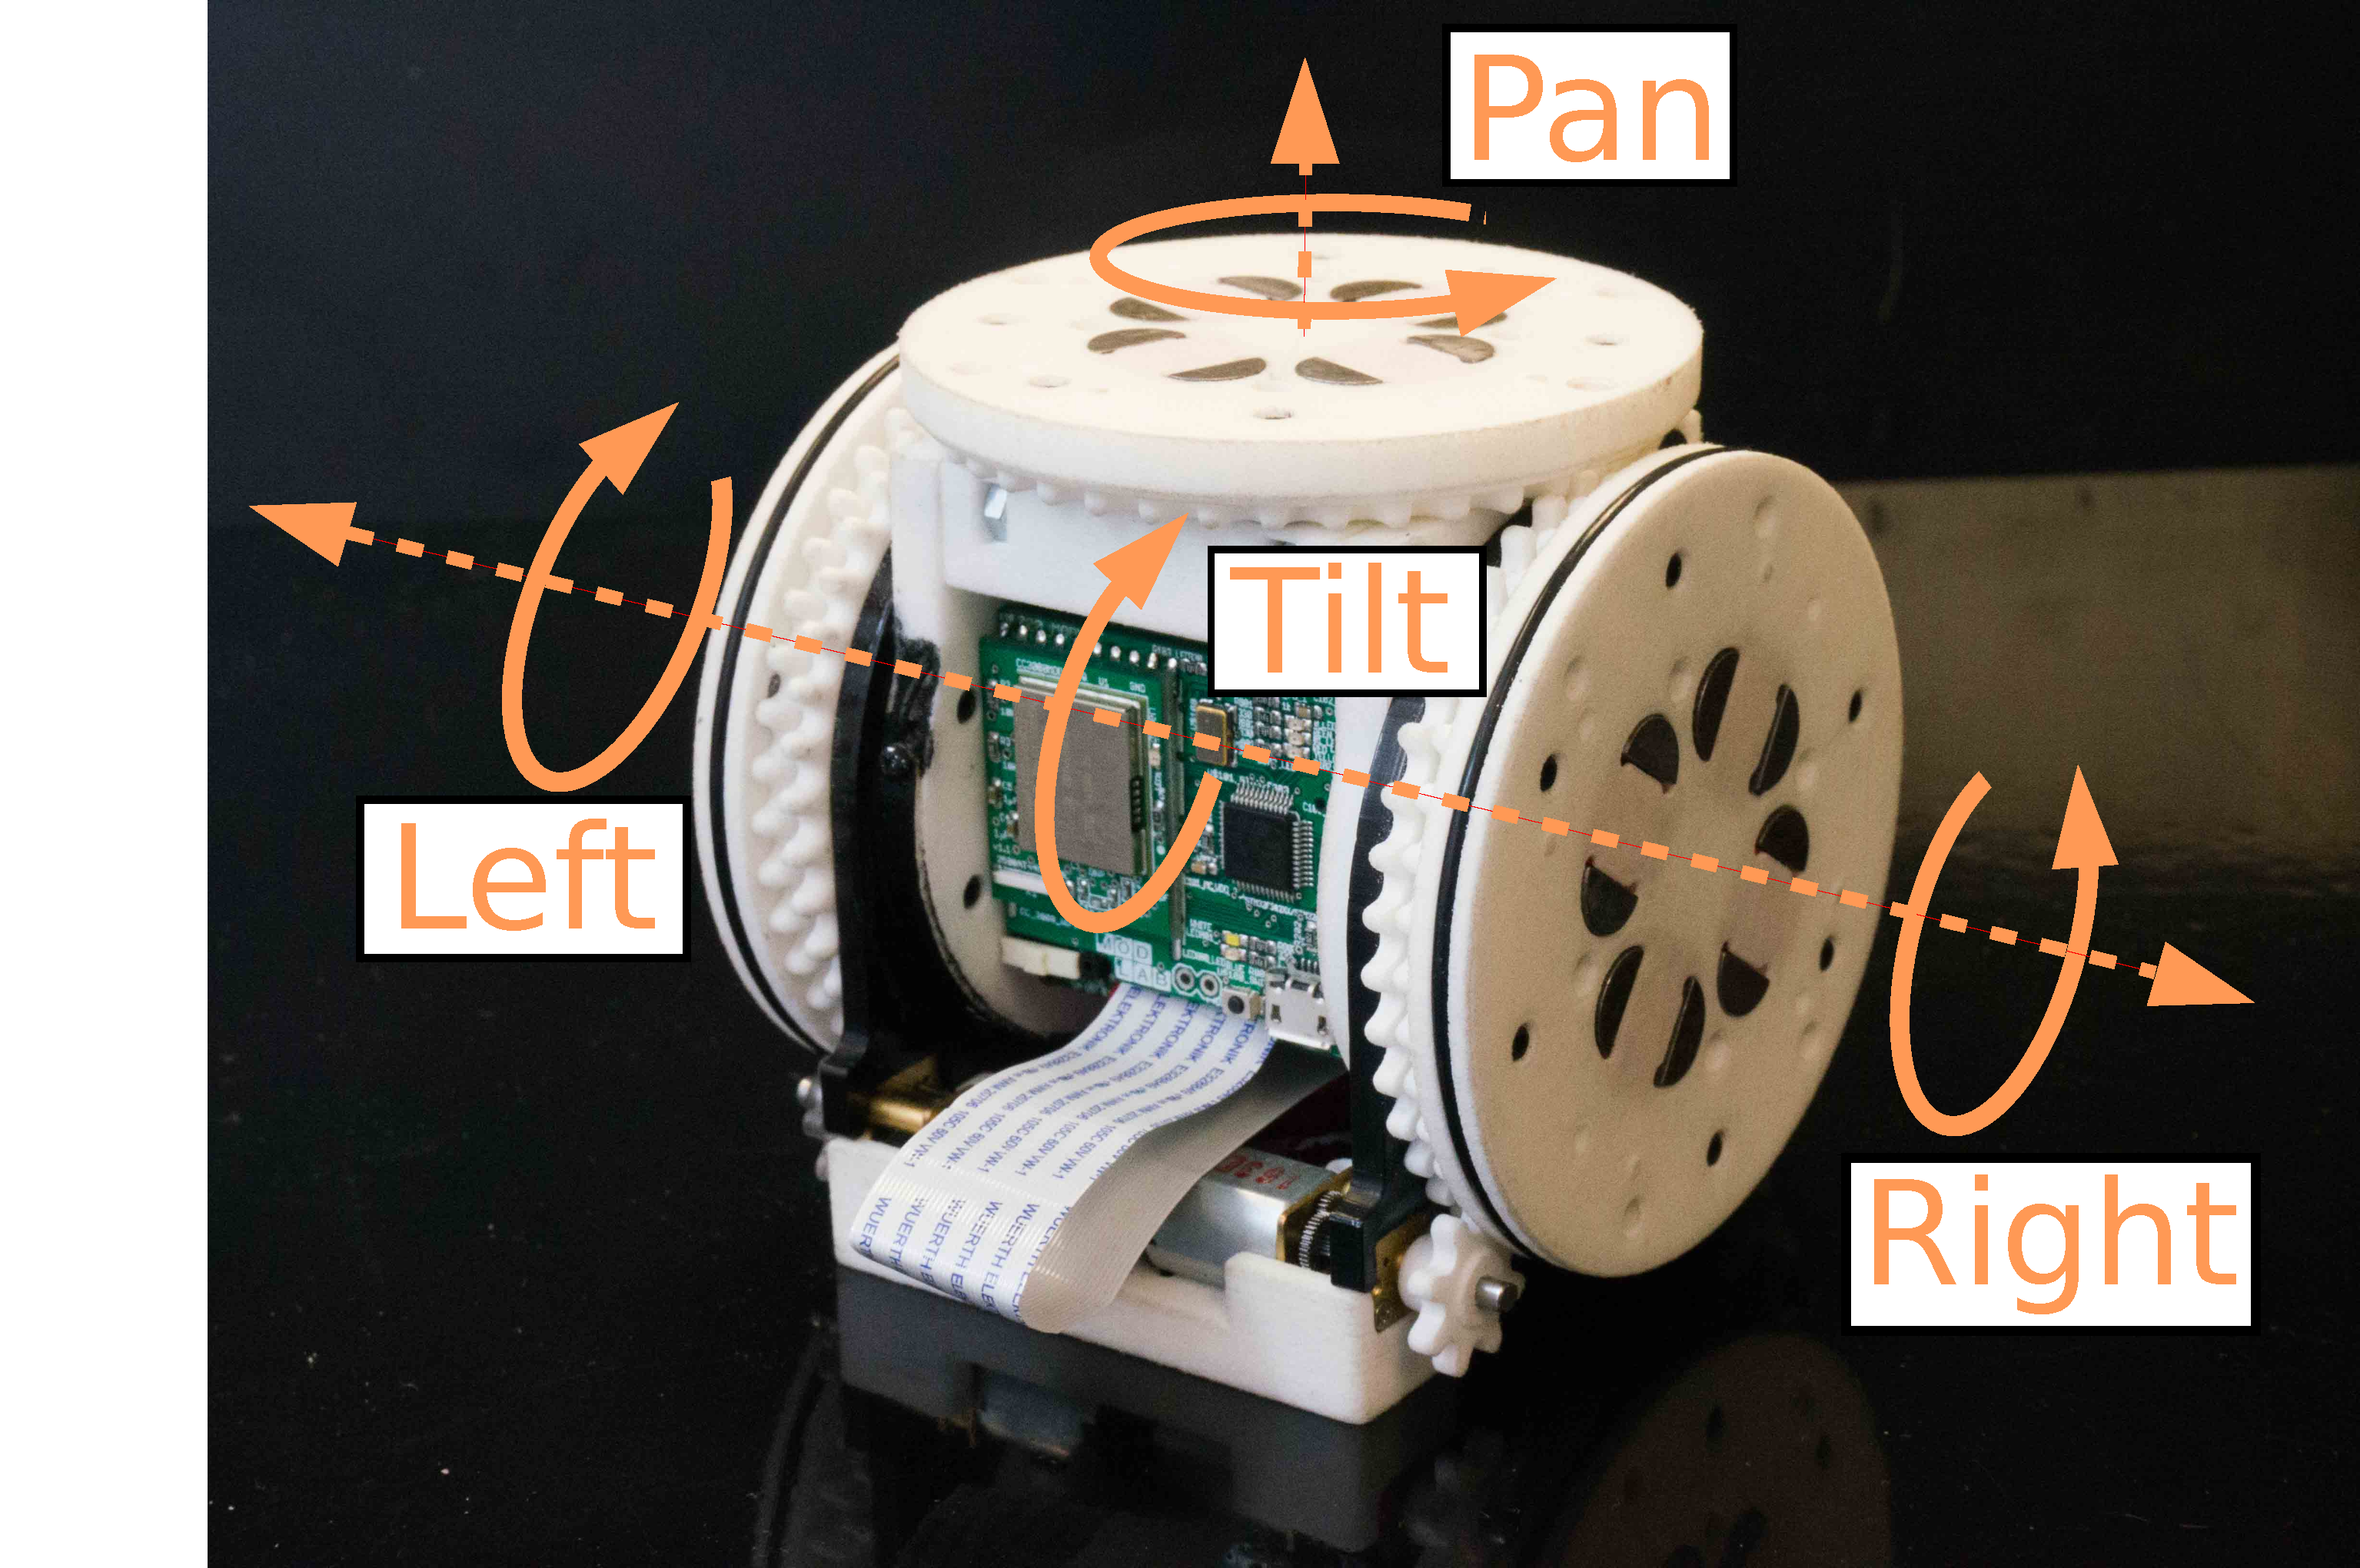
\includegraphics[height=1.5in]{images/smores_dof.pdf}
\end{center}
\caption{SMORES-EP module}
\label{fig:smores-module}
\end{figure}
%

\subsection{Sensor Module} % (fold)
\label{sec:sensor_module}
%

In MSRR systems, sensing and processing capabilities of individual modules are severely limited by the size and weight constraints of the module form factor. Therefore, the proposed system uses a special sensor module dedicated to sensing and processing equipment, shown in Figure \ref{fig:sensor-module}. The module has no actuation capabilities and is larger than SMORES-EP modules. It is equipped with a front-facing Xtion Pro Live RGB-D sensor\footnote{TODO: Xtion Ref} which enables the robot to explore and map the environment and recognize objects of interest. A high, downward-facing HD webcam is included to provide a view of the robot itself, which is used for self-reconfiguration. Finally, an UP computing board\footnote{TODO: Up Board Ref} provides high performance I/O and processing capability in a small form factor. The UP Board used in the proposed system has an Intel Atom 1.92 GHz processor, 4 GB memory, and a 64 GB hard drive. It is network connected via 802.11 wifi. A battery provides power to the Up Board with a lifetime of about 1.5 hours.

% Sensor Module Figure
\begin{figure}
\begin{center}
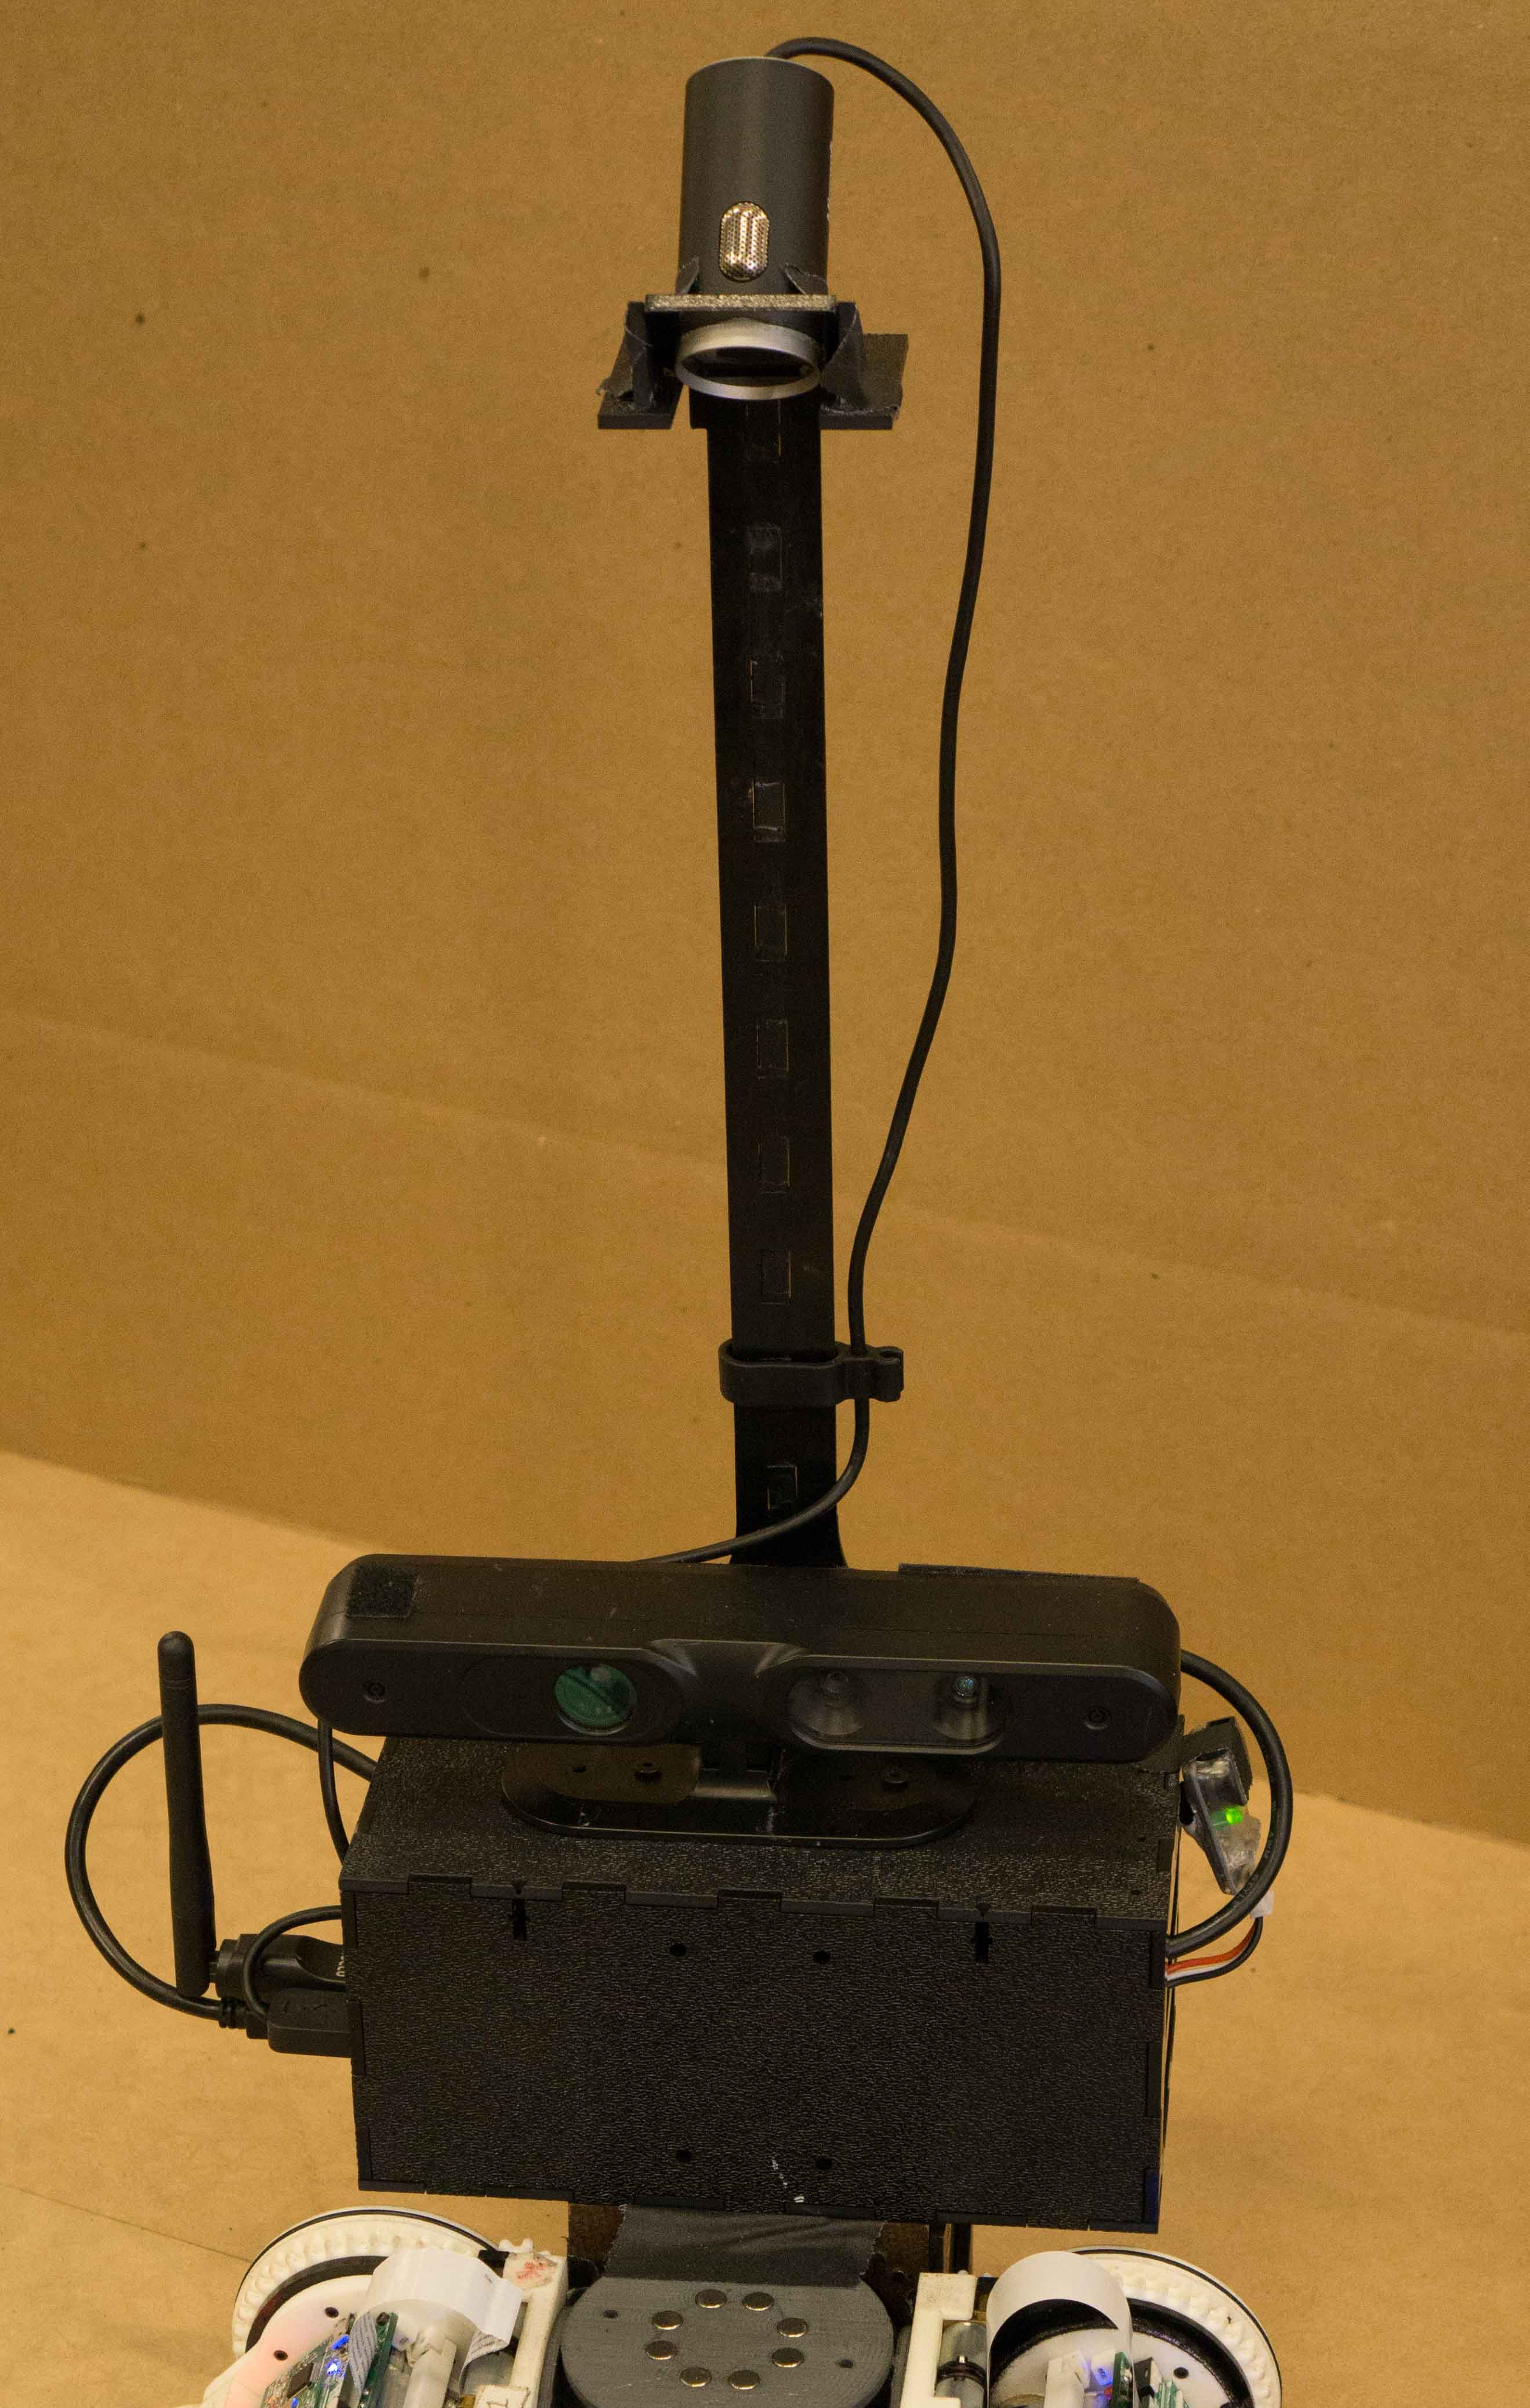
\includegraphics[width=0.4\textwidth]{images/sensor_module.jpg}
\caption{Sensor module. \TODO{get better picture}.}
\label{fig:sensor-module}
\end{center}
\end{figure}

%
% subsection sensor_module (end)
% section hardware (end)
%

\section{Perception and Environment Characterization}

\TODO{Yup yup yup}

\section{Configuration-Specific Controllers}

\TODO{All that low-level stuff}

\section{Reconfiguration}

\TODO{So robust...}

\section{High-Level Planner}

\TODO{Like, over 9000}

\section{Experimental Results}

\TODO{The impressive stuff}
\section{System Overview}

% Map
\begin{figure}
\begin{center}
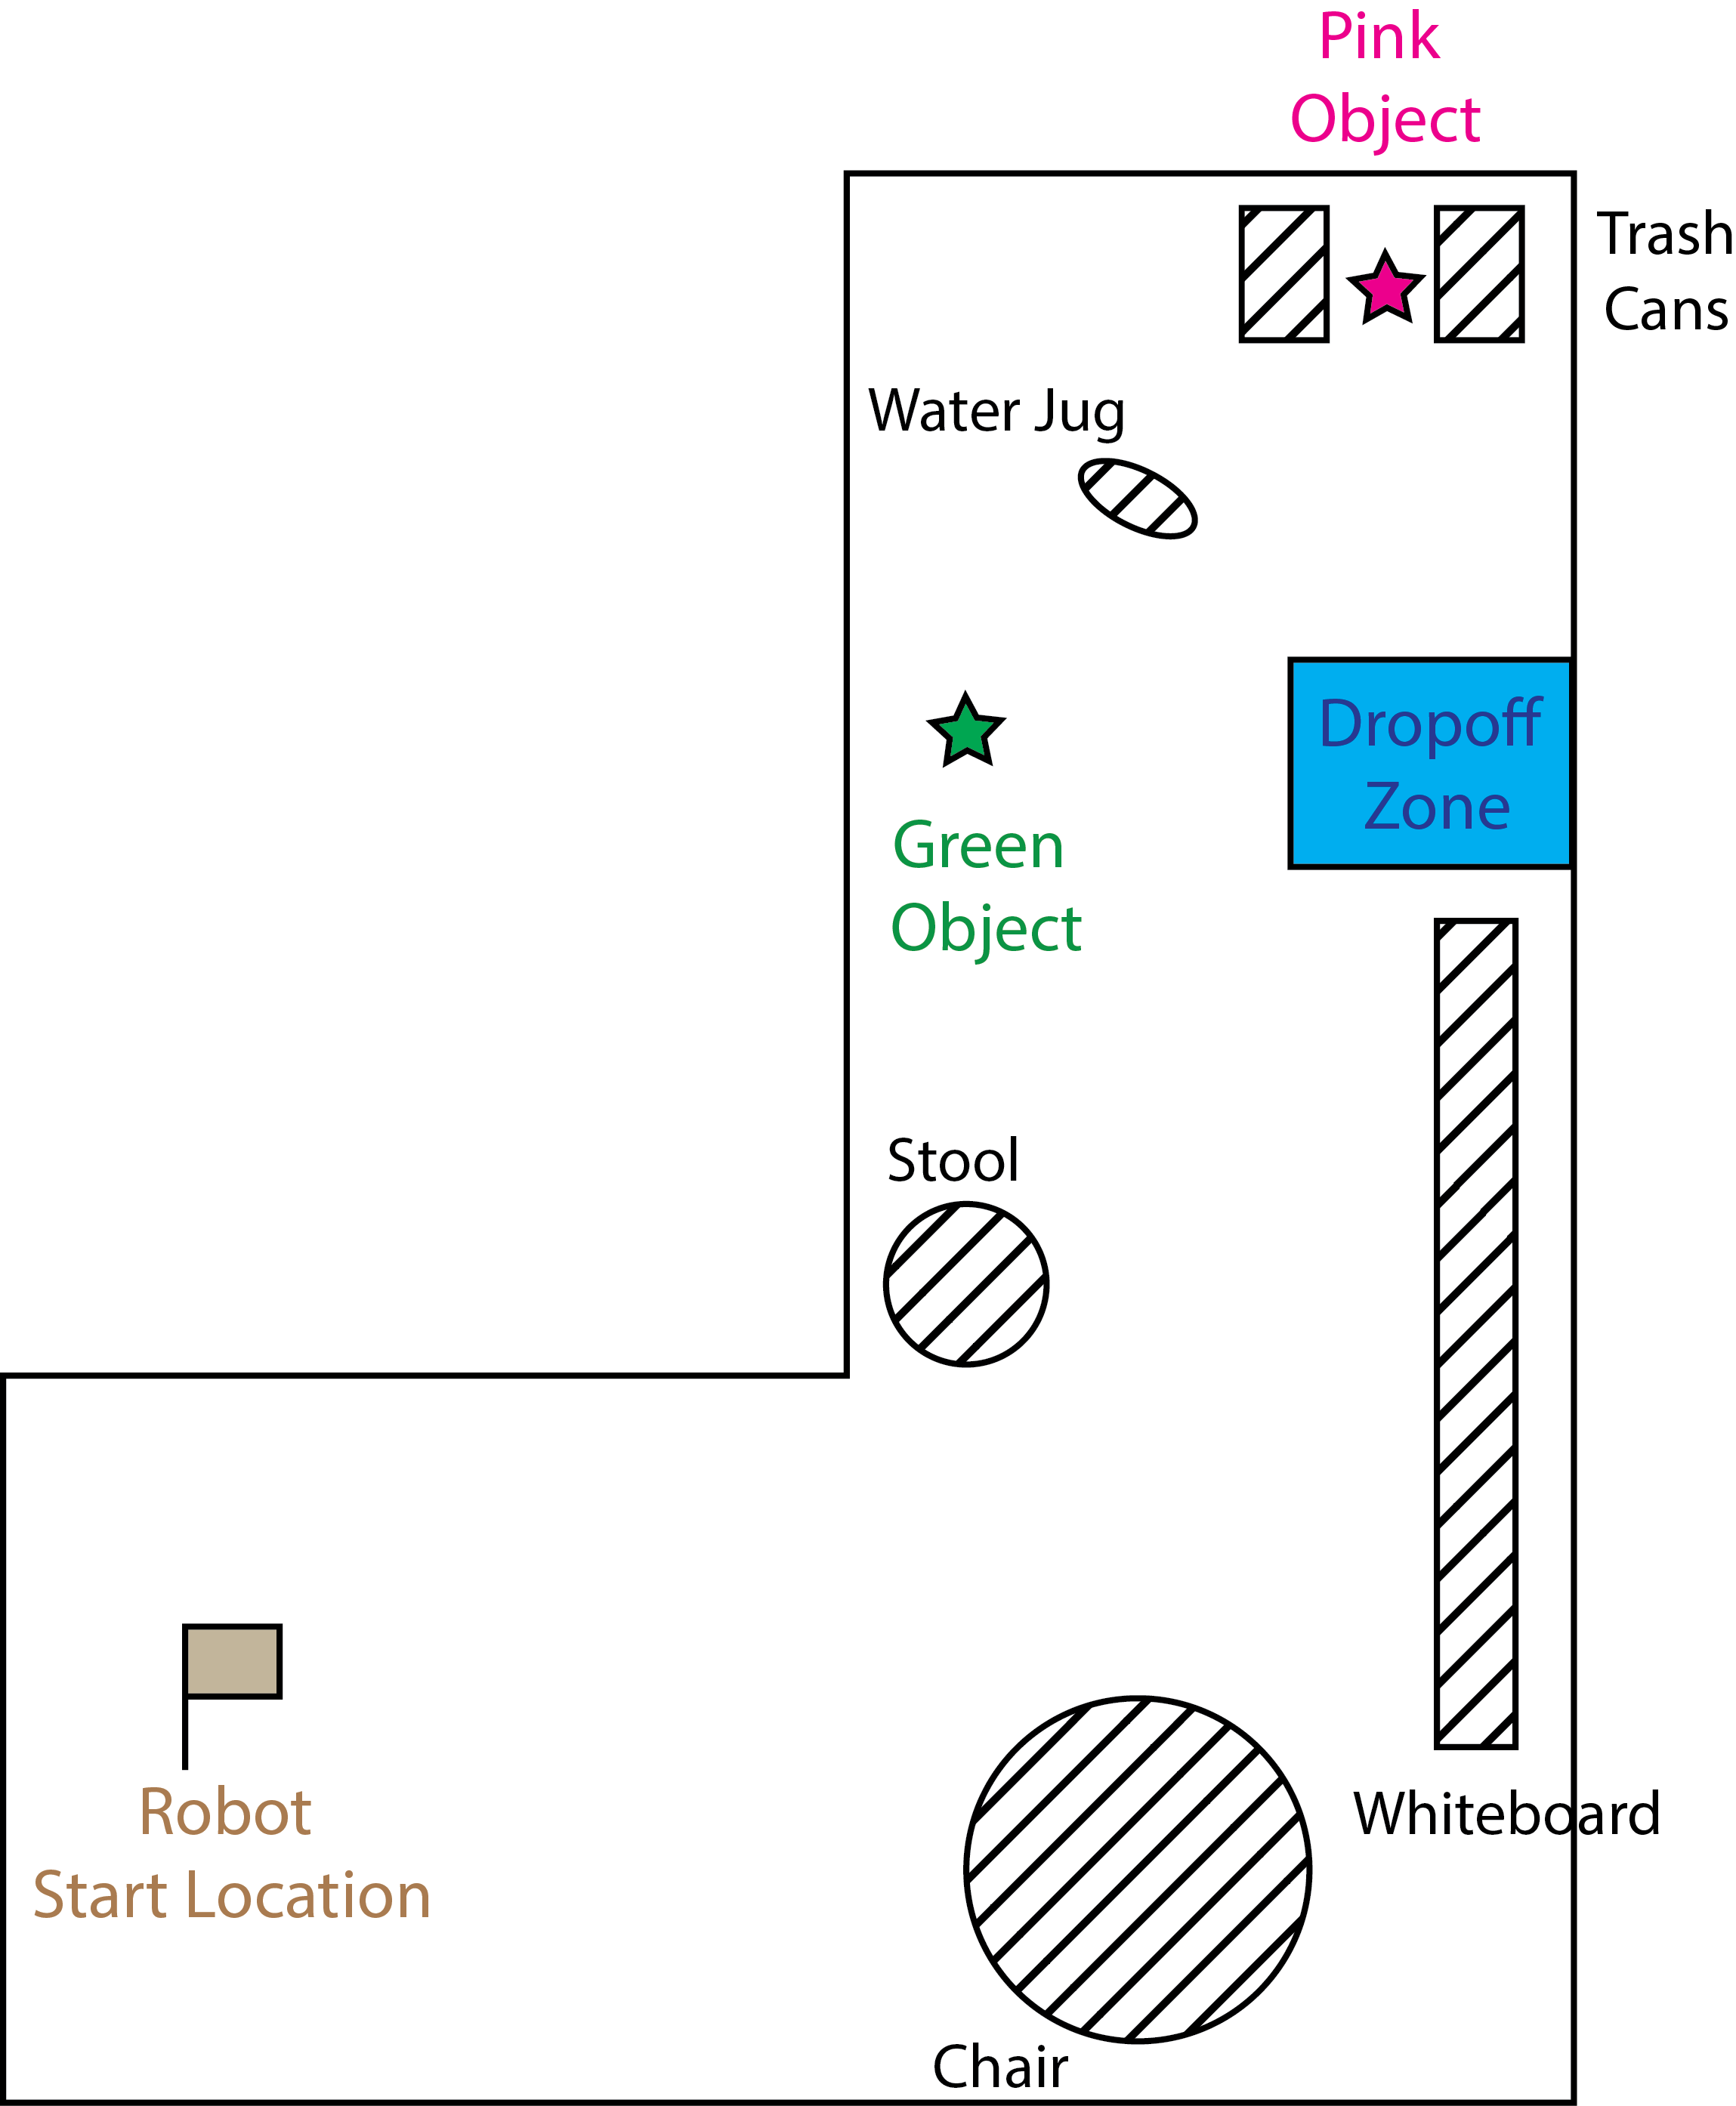
\includegraphics[width=0.4\textwidth]{images/RSSMap.png}
\caption{Experiment Map}
\label{fig:map}
\end{center}
\end{figure}

\section{Conclusion}

\TODO{Let's wrap this up}

\section*{Acknowledgments}
%
This work was funded by NSF grant numbers CNS-1329620 and CNS-1329692.
\TODO{Is this all of them?}


       %     ____       ____
       %    / __ \___  / __/__  ________  ____  ________  _____
       %   / /_/ / _ \/ /_/ _ \/ ___/ _ \/ __ \/ ___/ _ \/ ___/
       %  / _, _/  __/ __/  __/ /  /  __/ / / / /__/  __(__  )
       % /_/ |_|\___/_/  \___/_/   \___/_/ /_/\___/\___/____/

%% Use plainnat to work nicely with natbib. 
\bibliographystyle{plainnat}
\bibliography{references}

\end{document}












